\section{\hbadd{Evaluation on Different} Analysis Tasks}\label{sec:analysis-tasks}

\begin{table*}[t]
  \caption{Data sets used in experiments \duong{Update this table}}
  \centering
  \begin{tabular}{p{0.06\linewidth}p{0.24\linewidth}p{0.12\linewidth}p{0.05\linewidth}p{0.05\linewidth}p{0.05\linewidth}p{0.05\linewidth}p{0.06\linewidth}p{0.06\linewidth}p{0.06\linewidth}}
  \hline
  Name & Type & Dimension & Data type & Function & Gradient & Laplacian & Histogram & Isosurface & P or D\\
  \hline
  boiler & combustion simulation& $218\times 130 \times 150$ & float64 & x & x & x & x & x & Done \\
  plasma & magnetic reconnection simulation& $256\times 256 \times 256$ & float32 & x & x & x & x & x & P\\
  diffusivity & hydrodynamics simulation& $256\times 256\times 256$ & float64 & x & x & x & x & x & P\\
  pressure & hydrodynamics simulation& $256\times 256 \times 256$ & float64 & x & x & x & x & x & D(running)\\
  velocityz & hydrodynamics simulation& $256\times 256\times 256$ & float64 & x & x & x & x & x & Done\\
  turbulence & fluid dynamics simulation& $256\times 256 \times 256$ & float32 & x & x & x & x & x & P(running)\\
  kingsnake & fluid dynamics simulation& $256\times 256 \times 256$ & float32 & x & x & x & x & x & Done\\
  flame & fluid dynamics simulation& $256\times 256 \times 256$ & float32 & x & x & x & x & x & D(running)\\
  csafe & fluid dynamics simulation& $256\times 256 \times 256$ & float32 & x & x & x & x & x & D\\
  enzo-v & fluid dynamics simulation& $256\times 256 \times 256$ & float32 & x & x & x & x & x & D(running)\\
  brain & fluid dynamics simulation& $256\times 256 \times 256$ & uint16 & x & x & x & x & x & Done\\
  foam & fluid dynamics simulation& $256\times 256 \times 256$ & uint8 & x & x & x & x & x & P\\
  vismale & fluid dynamics simulation& $128\times 128 \times 128$ & uint8 & x & x & x & x & x & P\\
  karfs	& fluid dynamics simulation& $256\times 256 \times 256$ & float32 & x & x & x & x & x & D(running)\\
  \hline
  \end{tabular}\label{tbl:data-sets}
\end{table*}

In this section, we consider a variety of \hbadd{common} \hbdel{fundamental}
analysis tasks, namely function reconstruction (\Cref{sec:rmse-optimized}),
derivative computation (\Cref{sec:gradient,sec:laplacian}), histogram
computation (\Cref{sec:histogram}), and isocontour extraction
(\Cref{sec:isocontour}). For each task, we define an error metric $\err$ that
is the basis for evaluating the performance of different streams on the task.
We use~\Cref{alg:greedy} to compute a stream $\sopt$ that is optimized for each
task, and use its signature to compute $\ssig$.  We compare $\slvl$, $\sbit$,
$\swav$, $\smag$, $\ssig$, and $\sopt$ by evaluating the error as a function of
the number of packets received. To mimic the effects of entropy compression
commonly used in practice, we remove all packets that contain only leading zero
bits from each stream before plotting. This comparison is performed on a
variety of data sets, listed in \Cref{tbl:data-sets}. \todo{is the table going to stay?}
\duong{add the discussion
about reconstructing the whole data at full resolution before performing any
analysis task.}

\subsection{Function Reconstruction}\label{sec:rmse-optimized}

%\begin{figure}[t]
%\centering
% \subcaptionbox{\label{fig:rmse:boiler}\emph{boiler}}{{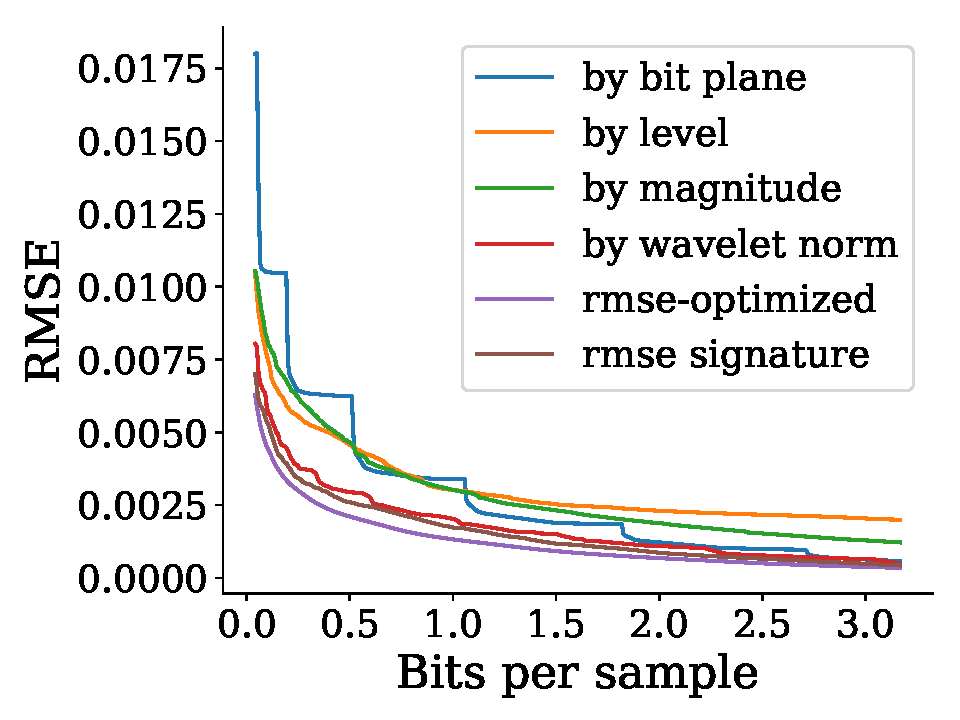
\includegraphics[width=0.48\linewidth]{rmse/rmse-optimized-boiler}}}
% \subcaptionbox{\label{fig:rmse:diffisivity}\emph{diffusivity}}{{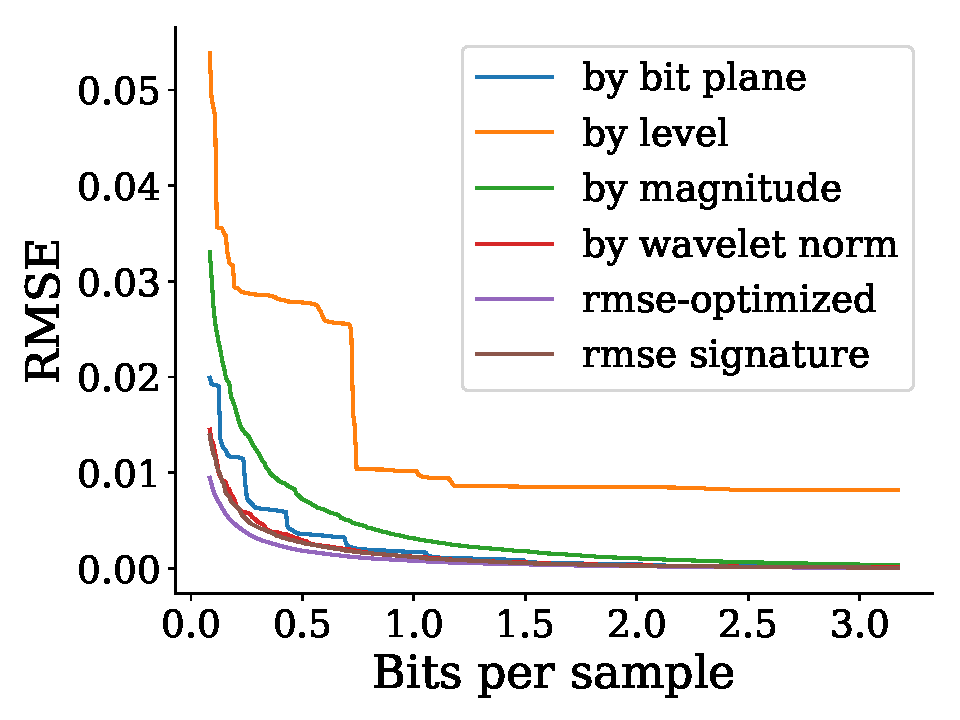
\includegraphics[width=0.48\linewidth]{rmse/rmse-optimized-diffusivity}}}
% \subcaptionbox{\label{fig:rmse:plasma}\emph{plasma}}{ {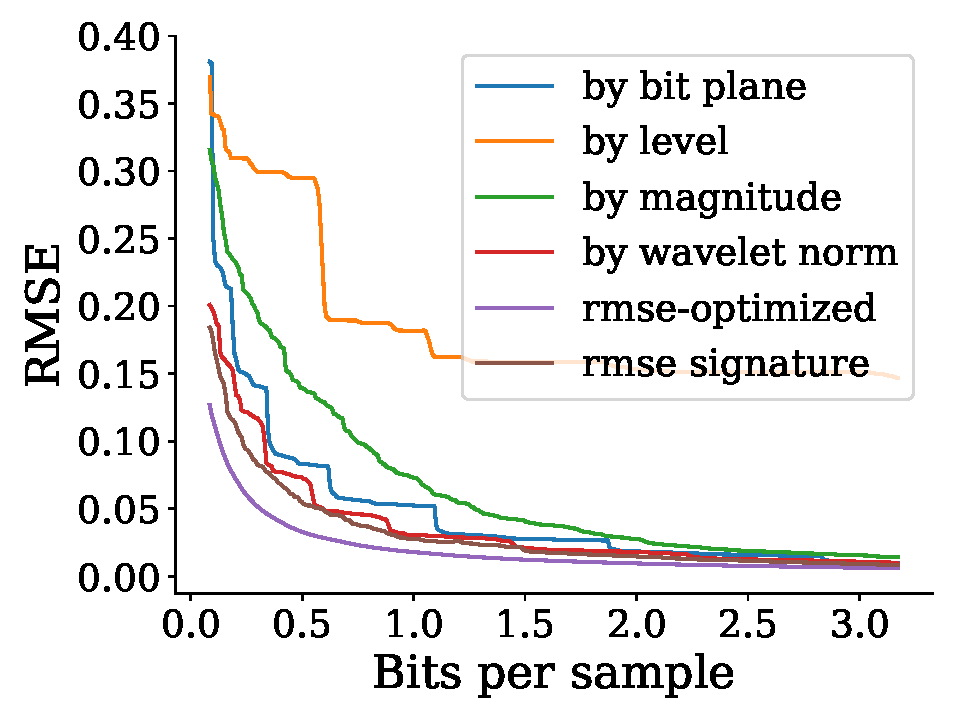
\includegraphics[width=0.48\linewidth]{rmse/rmse-optimized-plasma}}}
% \subcaptionbox{\label{fig:rmse:turbulence}\emph{turbulence}}{{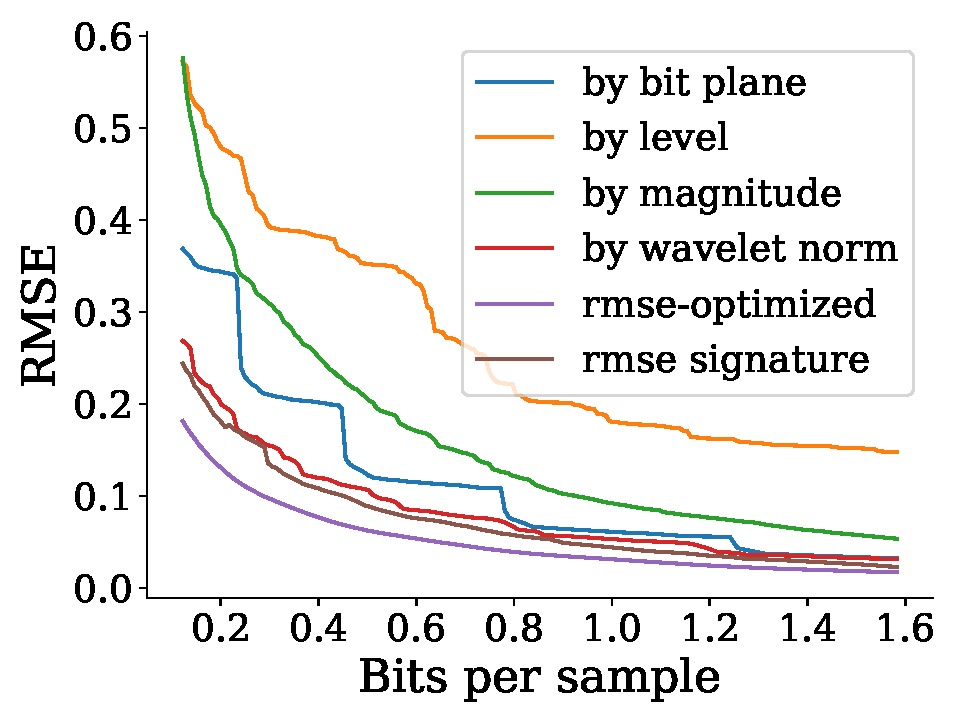
\includegraphics[width=0.48\linewidth]{rmse/rmse-optimized-turbulence}}}
%\caption{Root-mean-square error of reconstructed functions for different
%streams and data sets. The streams are truncated to highlight the differences,
%without omitting important information. Leading zero packets are not used for
%plotting. In all cases, the ordering of performance, from best to worst, is
%$\sopt > \ssig > \swav > \sbit > \smag > \slvl$.} \label{fig:rmse-optimized}
%\end{figure}
%
%\begin{figure}[t]
%\centering
% \subcaptionbox{\emph{by level} (\slvl)}{{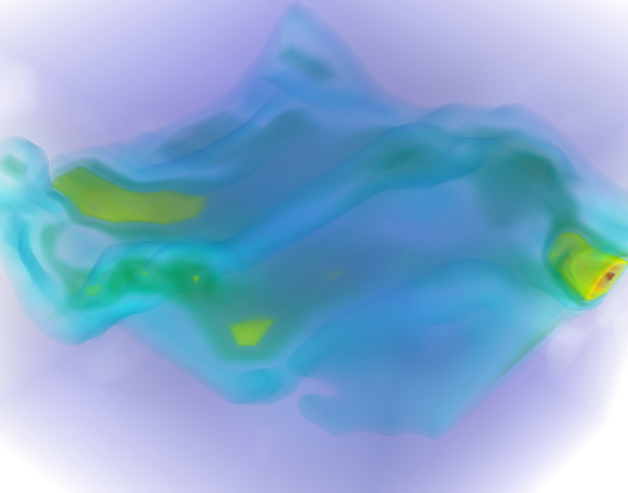
\includegraphics[width=0.32\linewidth]{rmse/rmse-plasma-level}}}
% \subcaptionbox{\emph{by bit plane (\sbit)}}{{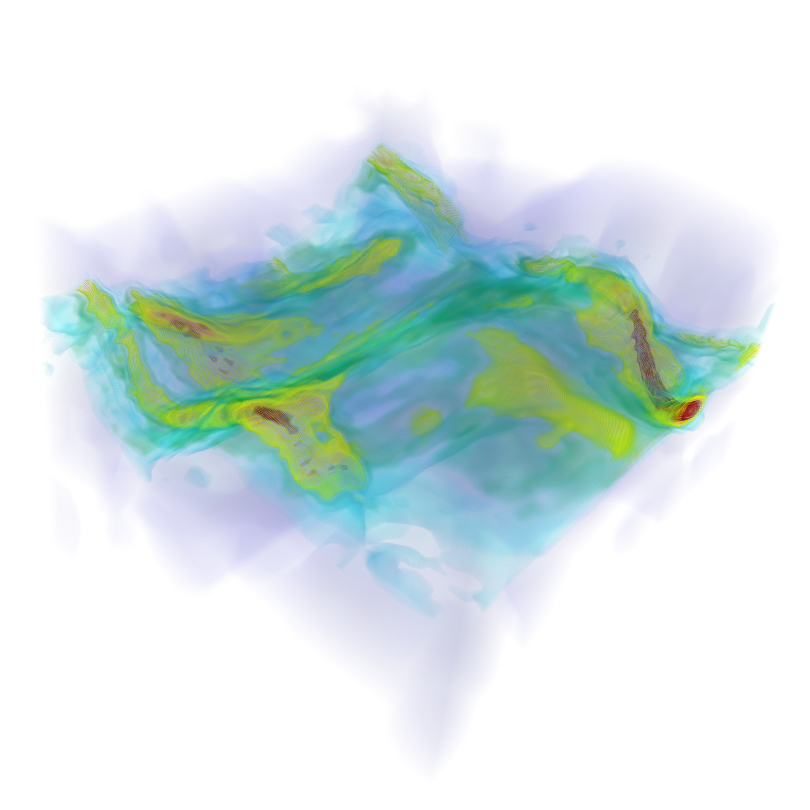
\includegraphics[width=0.32\linewidth]{rmse/rmse-plasma-bit-plane}}}
% \subcaptionbox{\emph{by wavelet norm (\swav)}}{{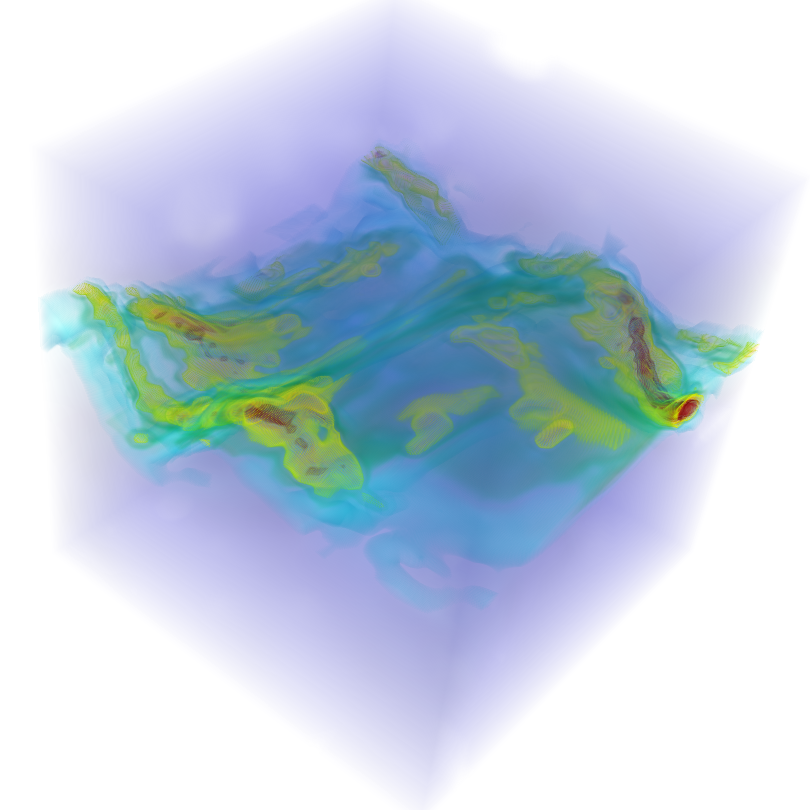
\includegraphics[width=0.32\linewidth]{rmse/rmse-plasma-wavelet-norm}}}
% \subcaptionbox{\emph{by magnitude (\smag)}}{{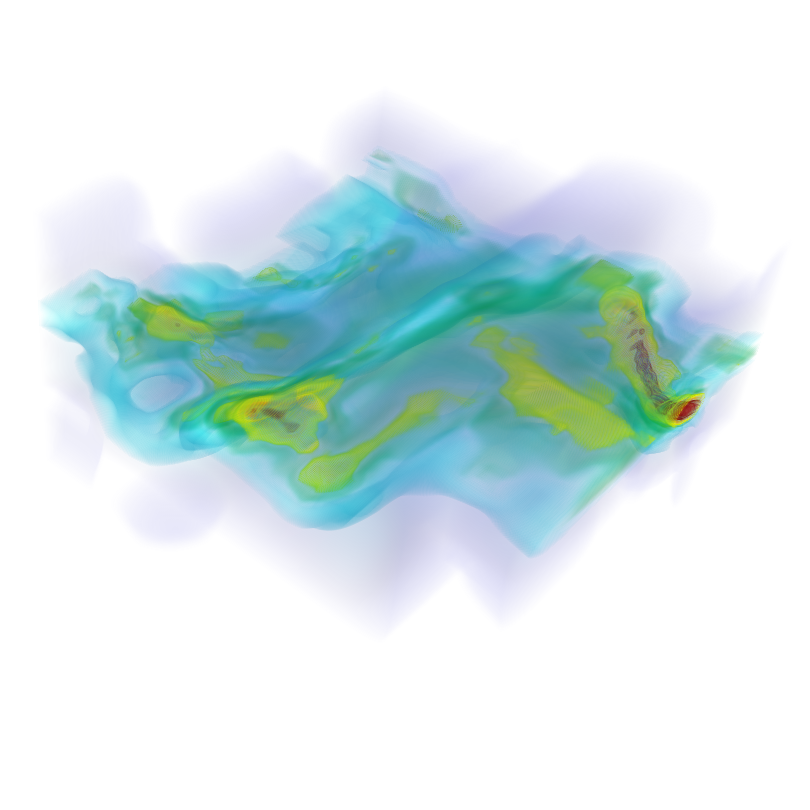
\includegraphics[width=0.32\linewidth]{rmse/rmse-plasma-magnitude}}}
% \subcaptionbox{\emph{by signature (\ssig)}}{{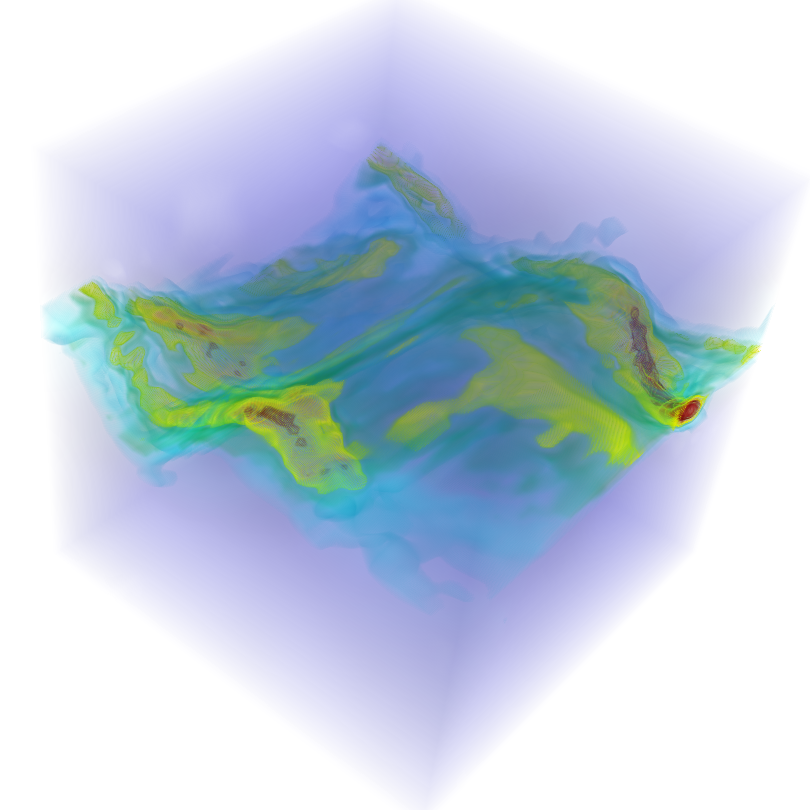
\includegraphics[width=0.32\linewidth]{rmse/rmse-plasma-signature}}}
% \subcaptionbox{\emph{ground truth}}{{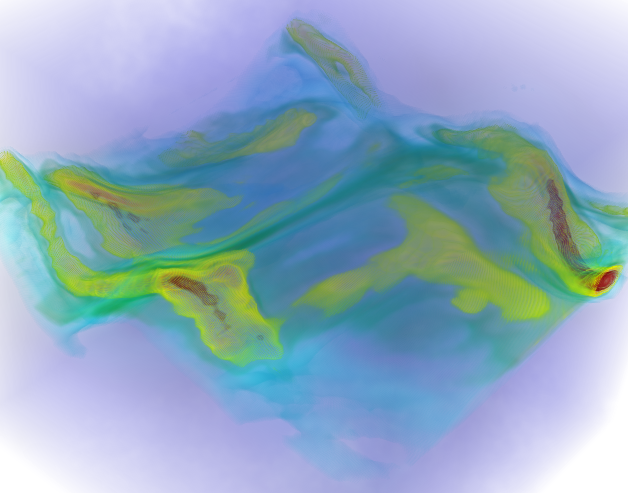
\includegraphics[width=0.32\linewidth]{rmse/rmse-plasma-groundtruth}}}
%\caption{Volume renderings of a $64^3$ region of \emph{plasma} data set at 0.1
%bps.  \slvl captures the background (purple-blue) well, whereas \sbit captures
%the fine details better. \swav combines the strength of both. \ssig, however,
%produces the most accurate rendering (compare, e.g., yellow features).
%\pavol{should we circle them or use an arrow?}\hb{yes, please}}
%\label{fig:rmse-rendering}
%\end{figure}

\begin{figure*}[t]
\centering
 \subcaptionbox{\label{fig:rmse:boiler}\emph{boiler}}{{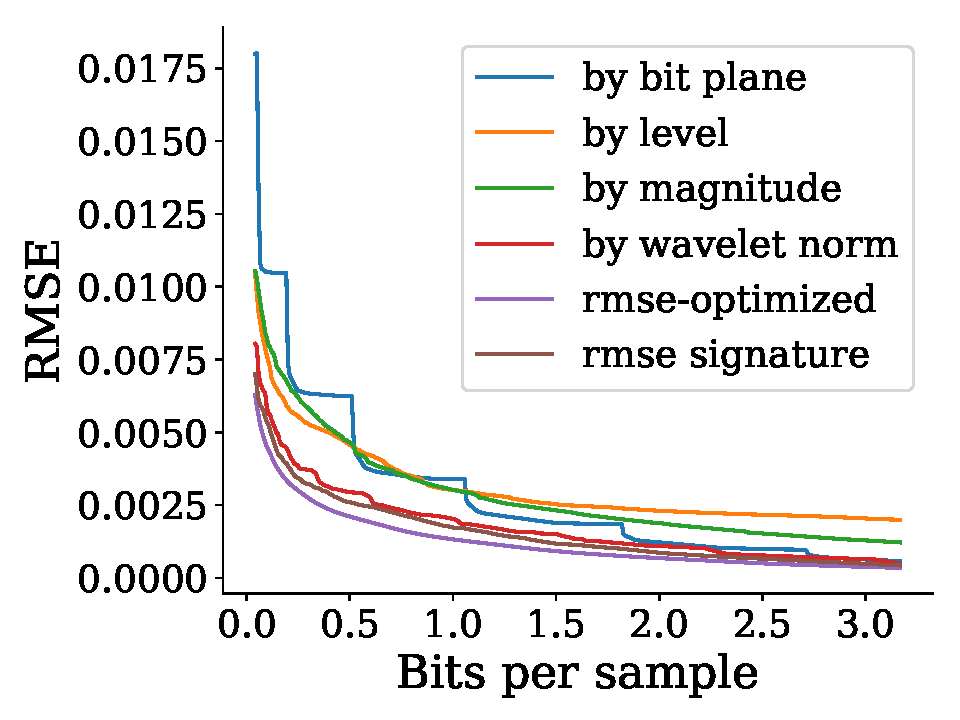
\includegraphics[width=0.24\linewidth]{rmse/rmse-optimized-boiler}}}
 \subcaptionbox{\label{fig:rmse:diffisivity}\emph{diffusivity}}{{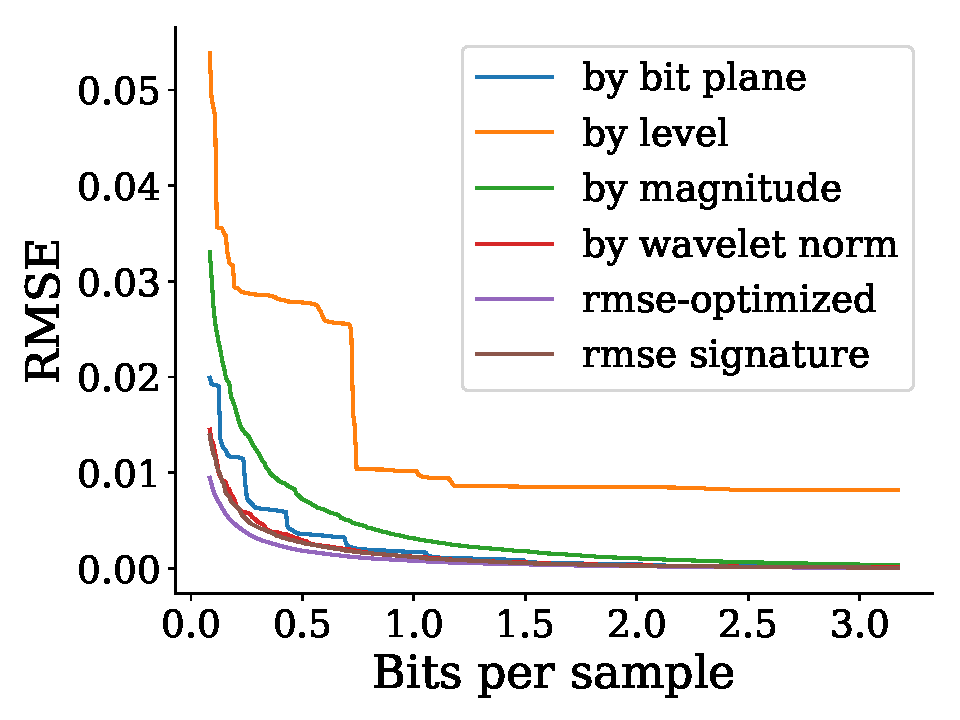
\includegraphics[width=0.24\linewidth]{rmse/rmse-optimized-diffusivity}}}
 \subcaptionbox{\label{fig:rmse:plasma}\emph{plasma}}{ {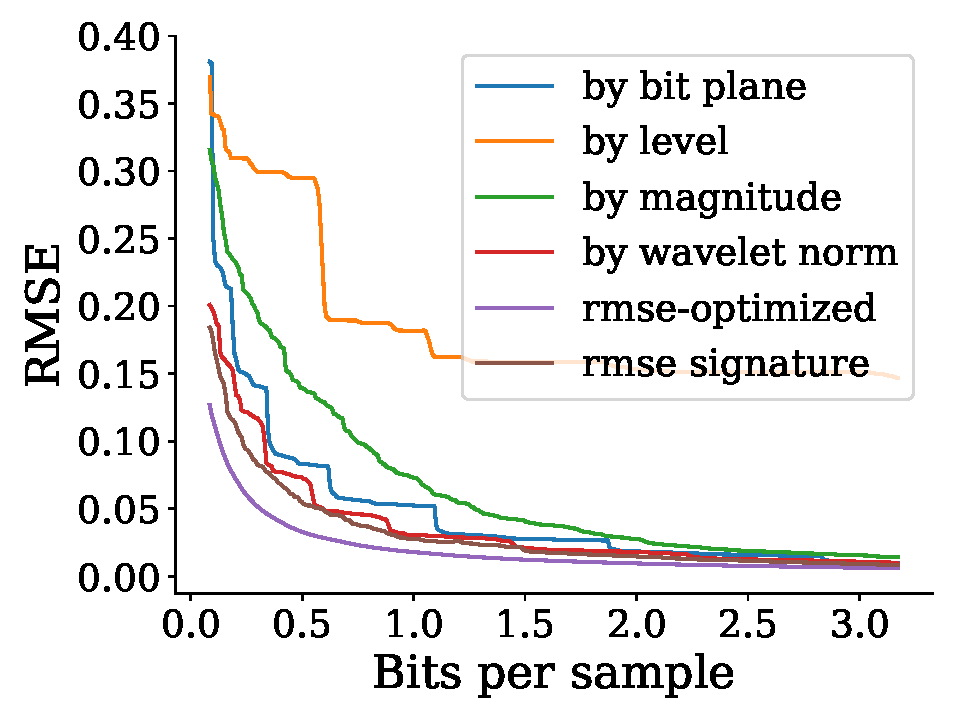
\includegraphics[width=0.24\linewidth]{rmse/rmse-optimized-plasma}}}
 \subcaptionbox{\label{fig:rmse:turbulence}\emph{turbulence}}{{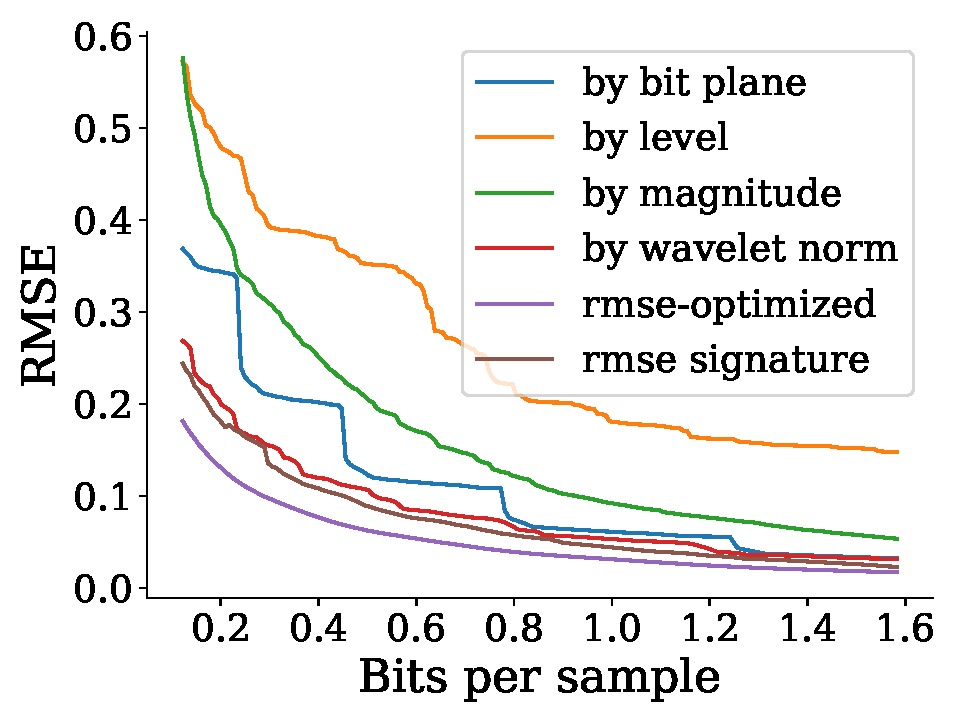
\includegraphics[width=0.24\linewidth]{rmse/rmse-optimized-turbulence}}}
\caption{Root-mean-square error (RMSE) of reconstructed functions for different
streams and data sets; lower RMSE is better. The streams are truncated to highlight the differences,
without omitting important information. Leading zero packets are not used for
plotting. In all cases, the ordering of performance, from best to worst, is
$\sopt > \ssig > \swav > \sbit > \smag > \slvl$.} \label{fig:rmse-optimized}
\vspace{1em}

\centering
 \subcaptionbox{\emph{by level} (\slvl)}{{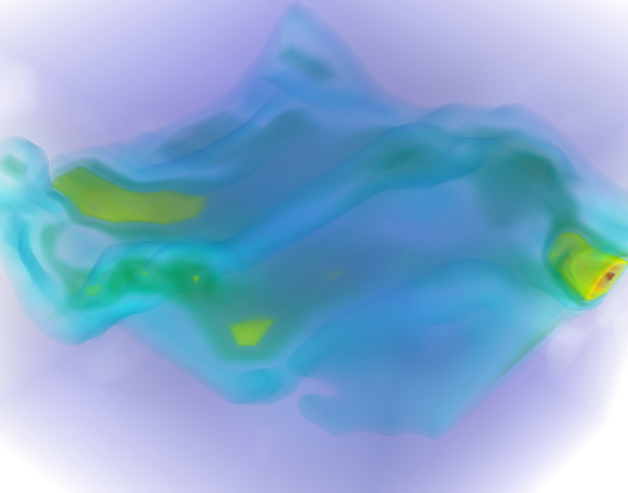
\includegraphics[width=0.16\linewidth]{rmse/rmse-plasma-level}}}
 \subcaptionbox{\emph{by bit plane (\sbit)}}{{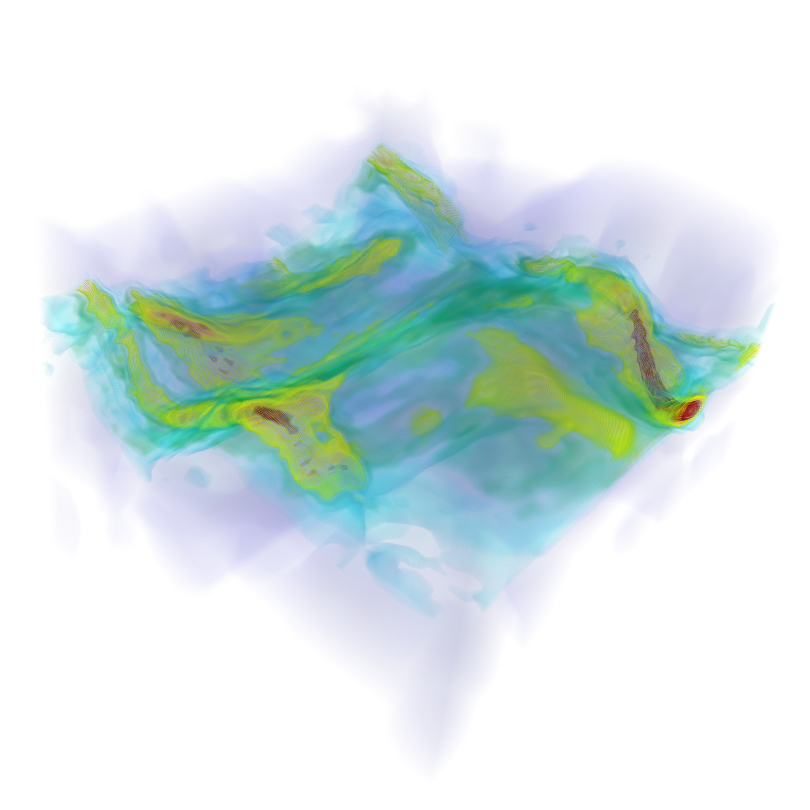
\includegraphics[width=0.16\linewidth]{rmse/rmse-plasma-bit-plane}}}
 \subcaptionbox{\emph{by wavelet norm (\swav)}}{{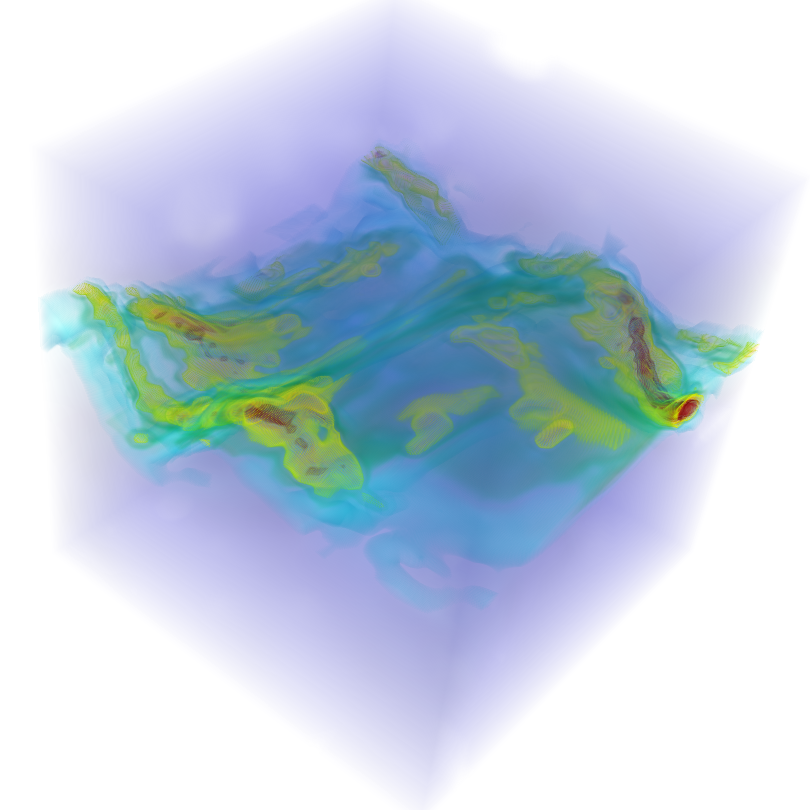
\includegraphics[width=0.16\linewidth]{rmse/rmse-plasma-wavelet-norm}}}
 \subcaptionbox{\emph{by magnitude (\smag)}}{{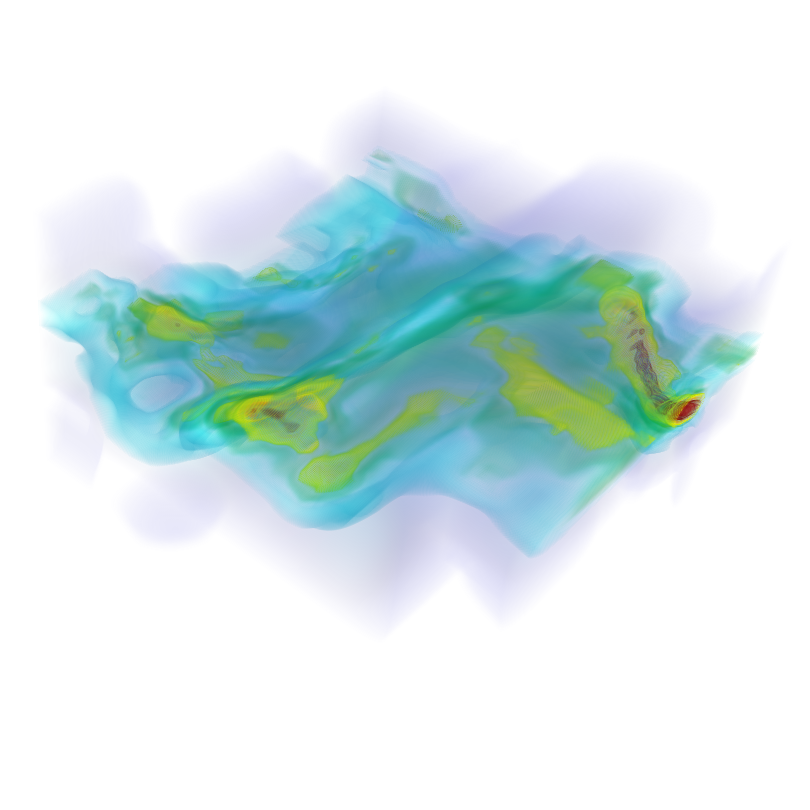
\includegraphics[width=0.16\linewidth]{rmse/rmse-plasma-magnitude}}}
 \subcaptionbox{\emph{by signature (\ssig)}}{{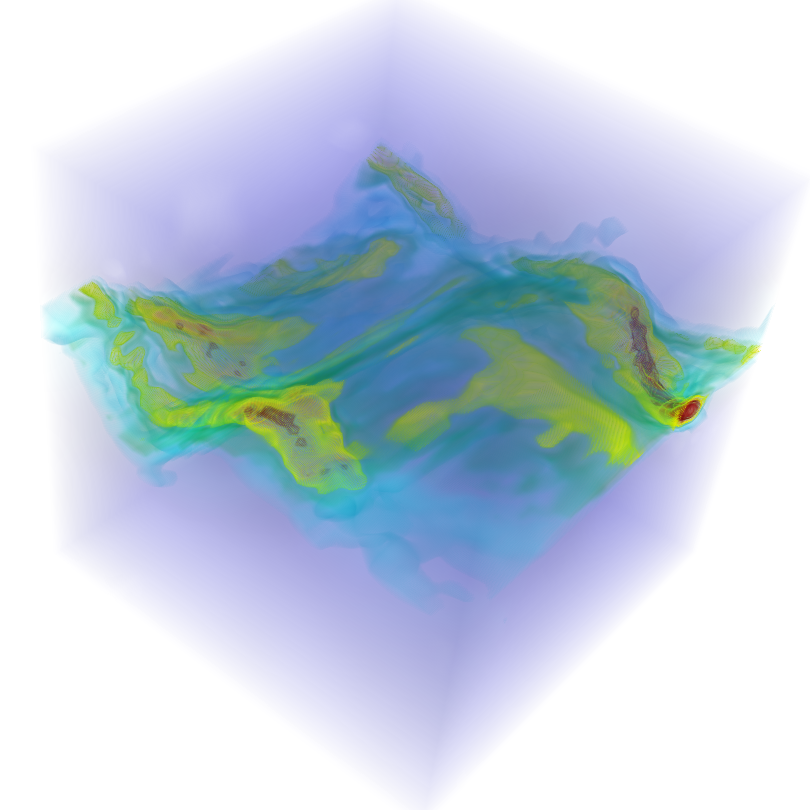
\includegraphics[width=0.16\linewidth]{rmse/rmse-plasma-signature}}}
 \subcaptionbox{\emph{ground truth}}{{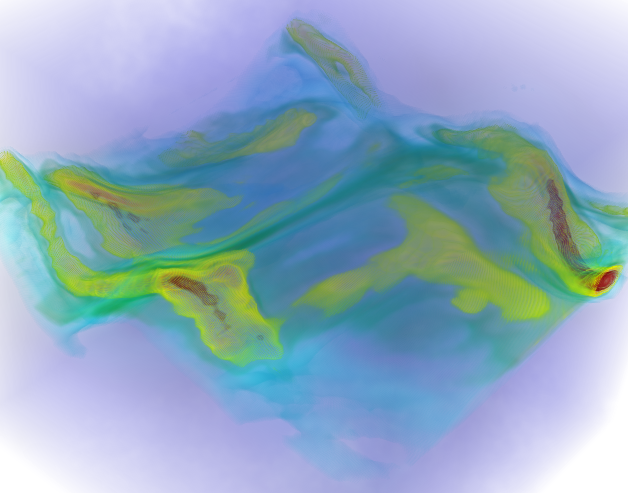
\includegraphics[width=0.16\linewidth]{rmse/rmse-plasma-groundtruth}}}
\caption{Volume renderings of a $64^3$ region of \emph{plasma} data set at 0.1
bps.  \slvl captures the background (purple-blue) well, whereas \sbit captures
the fine details better. \swav combines the strength of both. \ssig, however,
produces the most accurate rendering (compare, e.g., yellow features).
\pavol{should we circle them or use an arrow?}\hb{yes, please}}
\label{fig:rmse-rendering}
\end{figure*}

\hbadd{One of} the most fundamental analysis tasks is that of reconstructing
the original function itself.  \hbadd{A commonly used} \hbdel{The most common}
error metric in this case is the root-mean-square error (RMSE).
\hbadd{\autoref{fig:rmse-optimized} shows the comparison of the different
streams for a variety of datasets.  It can be noted that, in general, the
performance of the different streams are $\sopt > \ssig > \swav > \sbit > \smag
> \slvl$. Note that, better performance in this case is equivalent to producing
less RMSE.} \todo{DELETE: The plots that compare the streams are shown
in~\Cref{fig:rmse-optimized}. The main trend in all cases is $s_{opt} > s_{sig}
> s_{wav} > s_{bit} > s_{mag} > s_{lvl}$, where ``$>$'' means producing lower
RMSE errors. \pavol{counterintuitive} }

\hbadd{Furthermore,} \sbit performs significantly better than \slvl, which can
be attributed partly to our removal of leading zero packets, \hbdel{.
This\pavol{noun} is} because wavelet coefficients on finer scale subbands are
much smaller. \hbadd{Such coefficients} \hbdel{They} contain \hbadd{a}
\hbdel{the} majority of the leading zero bits, whose removal benefits \sbit the
most, as it touches fine-resolution bits the earliest. \smag underperforms for
the same reason that \slvl does, but to a lesser extent, \hbadd{since \smag is}
\hbdel{due to it being} better adaptive to the data. \swav outperforms both
\slvl and \sbit, because it follows the optimal (data-independent) bit ordering
in $\strm_{L,B}$ in the $L_2$ norm, which is also the norm that RMSE is based
upon. \hbadd{Unsurprisingly,} \sopt \hbdel{unsurprisingly} outperforms the
\hbadd{others} \hbdel{rest}, \hbadd{as it is} \hbdel{being} the most
data-adaptive.  \ssig is the second best stream, as it follows the bit ordering
of \sopt in $\strm_{L,B}$. In general, \swav and \ssig \hbadd{have similar}
\hbdel{are close in their} performance. In some cases (e.g.,
\hbadd{\autoref{fig:rmse:diffisivity} and~\autoref{fig:rmse:plasma}}
\hbdel{\emph{plasma} and \emph{diffusivity}}), \ssig is able to adapt more to
the data, thus outperforming \swav by a larger margin. \pavol{caused by empty
space?}

We explore the errors visually by volume rendering the \emph{plasma} data set
at 0.1 bits per sample, for all streams~(\autoref{fig:rmse-rendering}). Bits
per sample (bps) are calculated by dividing the total size of received packets
(in bits) by the total number of samples. Although \slvl has the precision to
obtain an accurate background, it lacks resolution to resolve the fine details.
\sbit, instead, lacks the precision to reconstruct the (mostly smooth)
background, but has enough resolution to capture the fine details well. \swav
balances both precision and resolution, producing a more accurate picture as a
whole. In this case, the \ssig stream manages to produce the most accurate
rendering. In general, \ssig benefits more from ``anisotropic'' data, such as
\emph{plasma}, where most features lie on a thin ``surface''. For such data,
wavelet coefficients along one dimension are often larger compared to those
along other dimensions, which \sopt, and hence \ssig, can take advantage of,
but not \swav.
